\section{Første iteration}
På figur~\ref{fig:26V_ideal_output} ses simuleringens resultatet for outputtet med en indgangsspænding på 26V.
\begin{figure}[H]
	\center
	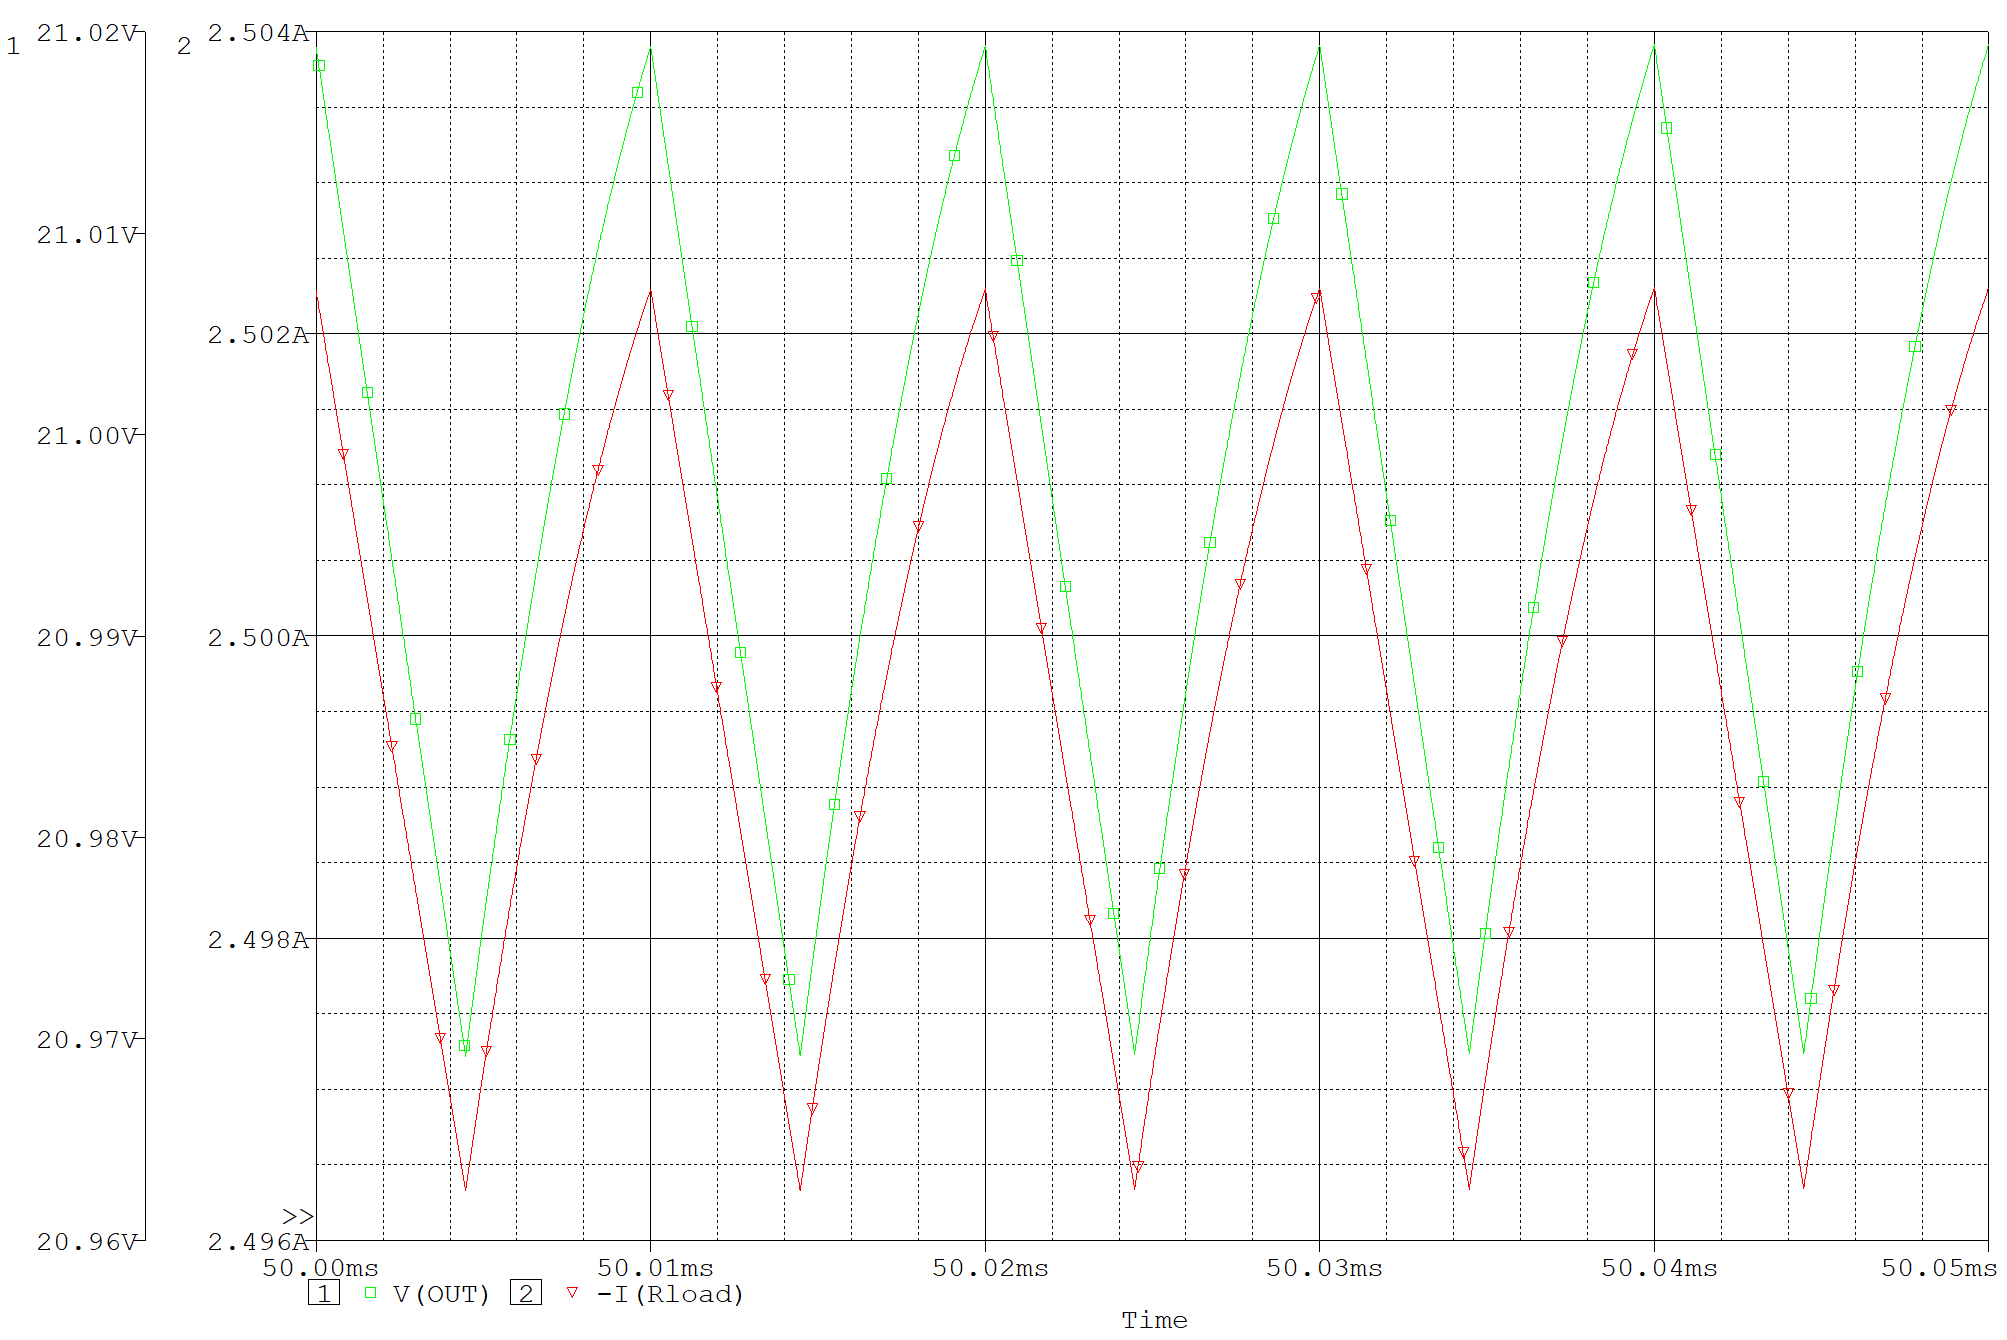
\includegraphics[max width=0.8\linewidth]{../dokumentation/tex/1iteration/billeder/26V_output.PNG}
	\caption{Converter output - ved 26V input}
	\label{fig:26V_ideal_output}
\end{figure}
Den grønne kurve er spændingen på outputtet, hvor y akse nummer et benyttes. Den røde kurve er udgangsstrømmen, hvor y akse nummer 2 benyttes.
 
Figur~\ref{fig:26V_transformer_current} viser hvordan strømmene løber i transformatoren, ved en inputspænding på 26V.
\begin{figure}[H]
	\center
	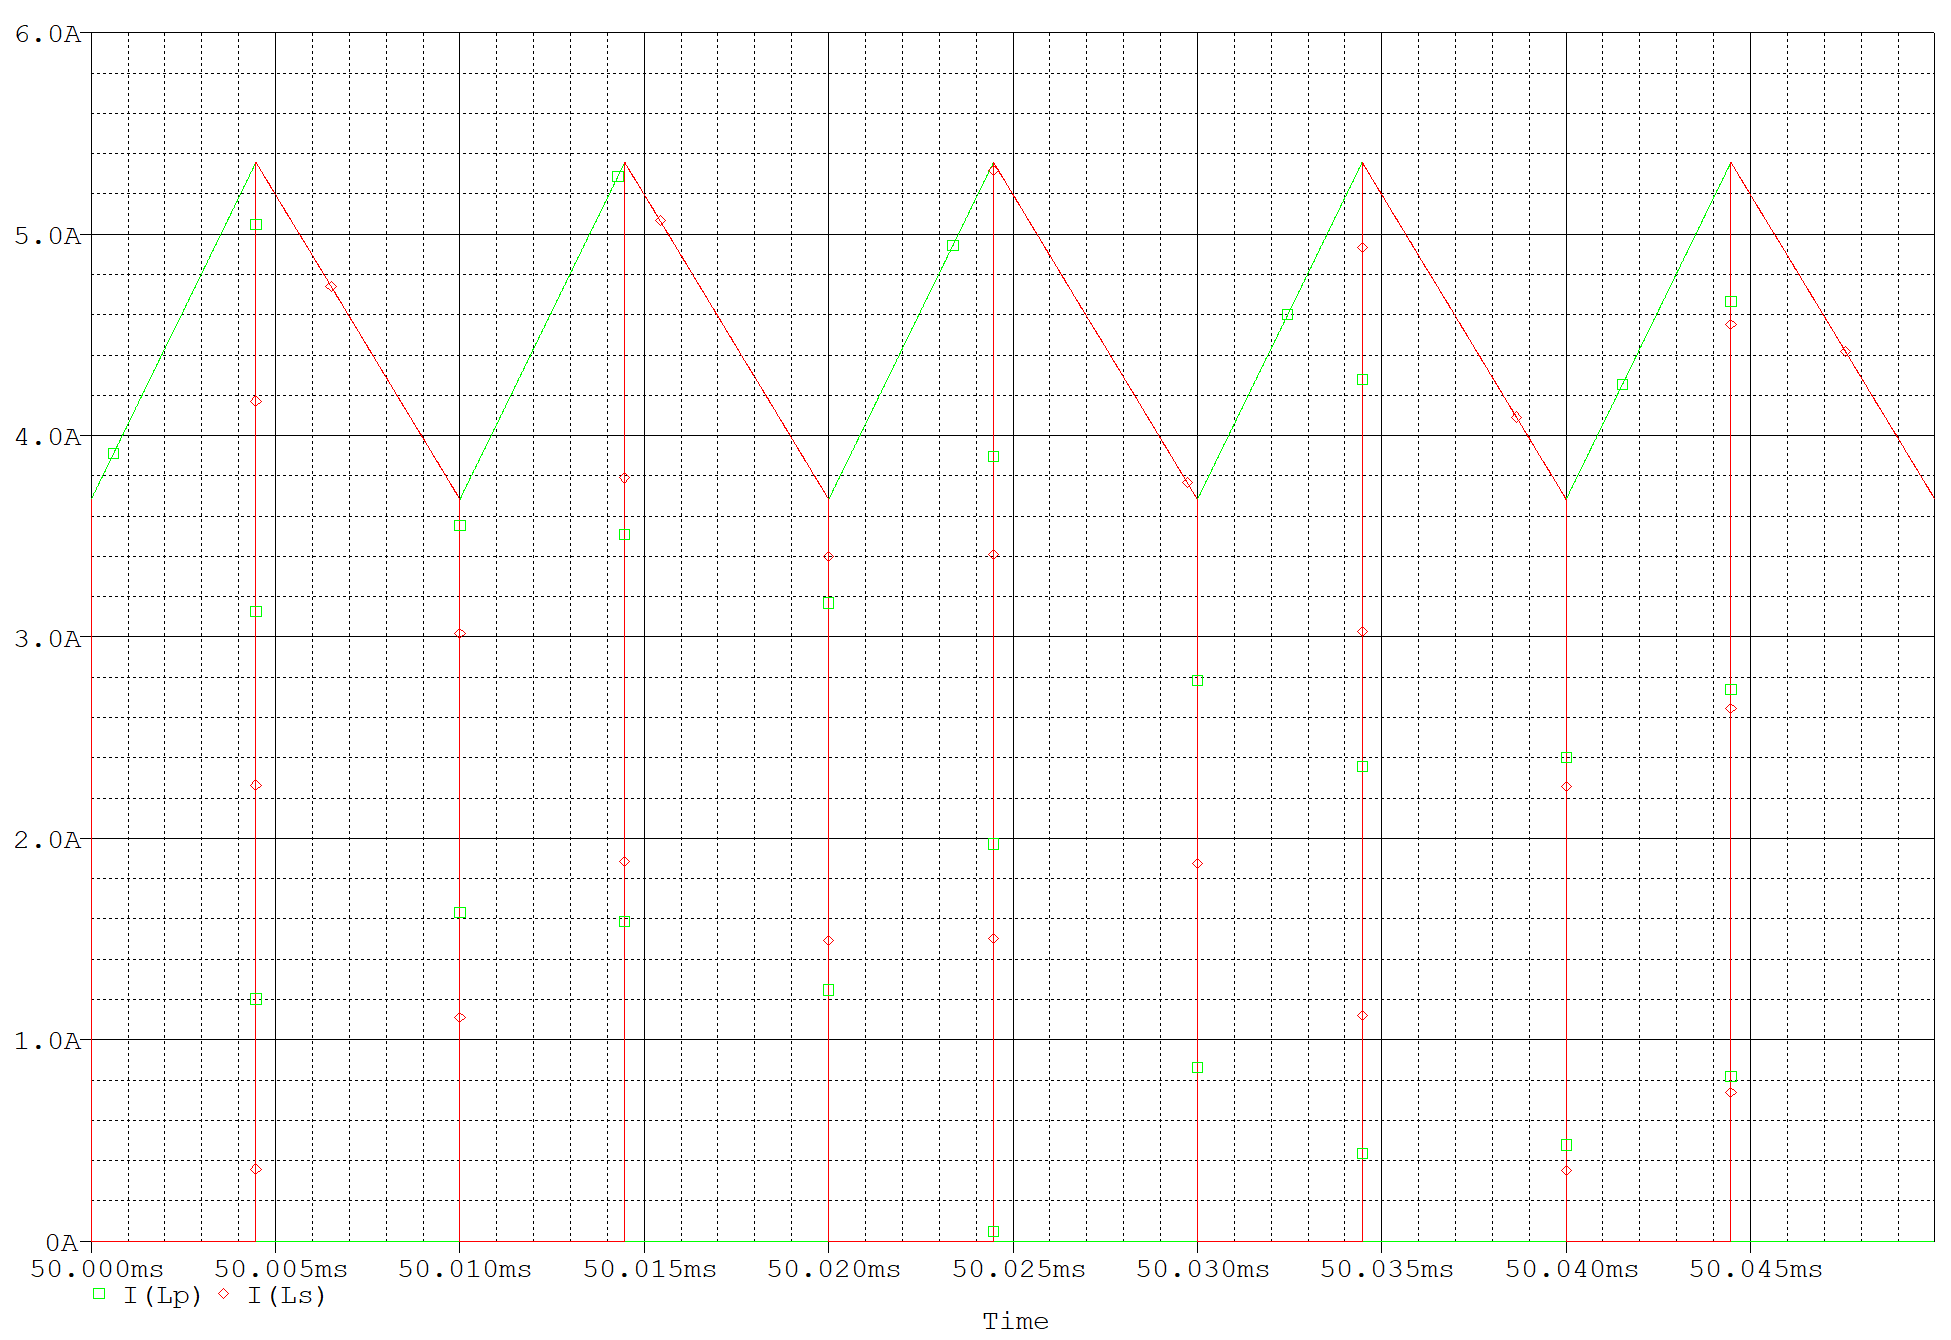
\includegraphics[max width=0.7\linewidth]{../dokumentation/tex/1iteration/billeder/26V_transformer_current.PNG}
	\caption{Transformator strømme - ved 26V input}
	\label{fig:26V_transformer_current}
\end{figure}
Den grønne kurve er strømmen i primærviklingen, mens den røde er viser strømmen i sekundærviklingen.

Tabel~\ref{tab:result_ideal_converter} viser de vigtigste beregnede og simulerede strømme for den ideele converter med indgangsspændinger på 26V og 50V. Tabellen bruges til at sammenligne, hvor godt de brugte udregninger stemmer overens med simuleringen.

\begin{table}[H] 			
	\centering
	\begin{tabularx}{\textwidth}{|X|c|c|c|c|c|c|c|c|}
		\hline
		\textbf{Indgangs-spænding} & \multicolumn{2}{|X|}{\textbf{Ripple-strøm}} & \multicolumn{2}{|X|}{\textbf{Peak-strøm}} & \multicolumn{2}{|X|}{\textbf{RMS-strøm i primær}} & \multicolumn{2}{|X|}{\textbf{RMS-strøm i sekundær}} \\ \hline
		& A & S & A & S & A & S & A & S \\ \hline
		$26V$ & $1.67A$ & $1.66A$ & $5.36A$ & $5.35A$ & $3.02A$ & $3.08A$ & $3.36A$ & $3.33A$ \\ \hline 
		$50V$ & $2.13A$ & $2.11A$ & $4.62A$ & $4.61A$ & $1.93A$ & $1.98A$ & $2.98A$ & $3.01A$ \\ \hline
	\end{tabularx}
	\caption{Resultater for analyse og simulering af ideel flyback converter}
	\label{tab:result_ideal_converter}
\end{table}